% Marking 1, 2, 3, ... on each fiber: the vector space structure.
% Source: book/tex/riemann-surface/line-bundles.tex (asy figure).
\documentclass[border=2mm]{standalone}
\usepackage{tikz}
\begin{document}
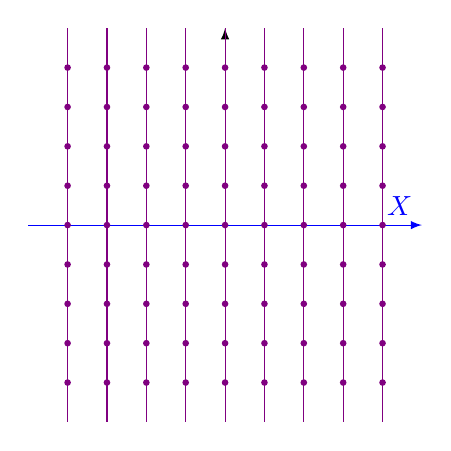
\begin{tikzpicture}[scale=0.5,>=latex]
  \draw[blue,->] (-5,0) -- (5,0) node[anchor=south east] {$X$};
  \draw[->] (0,-5) -- (0,5);
  \draw[violet] (-4,-5) -- (-4,5);
  \fill[violet] (-4,-4) circle (2.4pt);
  \fill[violet] (-4,-3) circle (2.4pt);
  \fill[violet] (-4,-2) circle (2.4pt);
  \fill[violet] (-4,-1) circle (2.4pt);
  \fill[violet] (-4,0) circle (2.4pt);
  \fill[violet] (-4,1) circle (2.4pt);
  \fill[violet] (-4,2) circle (2.4pt);
  \fill[violet] (-4,3) circle (2.4pt);
  \fill[violet] (-4,4) circle (2.4pt);
  \draw[violet] (-3,-5) -- (-3,5);
  \fill[violet] (-3,-4) circle (2.4pt);
  \fill[violet] (-3,-3) circle (2.4pt);
  \fill[violet] (-3,-2) circle (2.4pt);
  \fill[violet] (-3,-1) circle (2.4pt);
  \fill[violet] (-3,0) circle (2.4pt);
  \fill[violet] (-3,1) circle (2.4pt);
  \fill[violet] (-3,2) circle (2.4pt);
  \fill[violet] (-3,3) circle (2.4pt);
  \fill[violet] (-3,4) circle (2.4pt);
  \draw[violet] (-2,-5) -- (-2,5);
  \fill[violet] (-2,-4) circle (2.4pt);
  \fill[violet] (-2,-3) circle (2.4pt);
  \fill[violet] (-2,-2) circle (2.4pt);
  \fill[violet] (-2,-1) circle (2.4pt);
  \fill[violet] (-2,0) circle (2.4pt);
  \fill[violet] (-2,1) circle (2.4pt);
  \fill[violet] (-2,2) circle (2.4pt);
  \fill[violet] (-2,3) circle (2.4pt);
  \fill[violet] (-2,4) circle (2.4pt);
  \draw[violet] (-1,-5) -- (-1,5);
  \fill[violet] (-1,-4) circle (2.4pt);
  \fill[violet] (-1,-3) circle (2.4pt);
  \fill[violet] (-1,-2) circle (2.4pt);
  \fill[violet] (-1,-1) circle (2.4pt);
  \fill[violet] (-1,0) circle (2.4pt);
  \fill[violet] (-1,1) circle (2.4pt);
  \fill[violet] (-1,2) circle (2.4pt);
  \fill[violet] (-1,3) circle (2.4pt);
  \fill[violet] (-1,4) circle (2.4pt);
  \draw[violet] (0,-5) -- (0,5);
  \fill[violet] (0,-4) circle (2.4pt);
  \fill[violet] (0,-3) circle (2.4pt);
  \fill[violet] (0,-2) circle (2.4pt);
  \fill[violet] (0,-1) circle (2.4pt);
  \fill[violet] (0,0) circle (2.4pt);
  \fill[violet] (0,1) circle (2.4pt);
  \fill[violet] (0,2) circle (2.4pt);
  \fill[violet] (0,3) circle (2.4pt);
  \fill[violet] (0,4) circle (2.4pt);
  \draw[violet] (1,-5) -- (1,5);
  \fill[violet] (1,-4) circle (2.4pt);
  \fill[violet] (1,-3) circle (2.4pt);
  \fill[violet] (1,-2) circle (2.4pt);
  \fill[violet] (1,-1) circle (2.4pt);
  \fill[violet] (1,0) circle (2.4pt);
  \fill[violet] (1,1) circle (2.4pt);
  \fill[violet] (1,2) circle (2.4pt);
  \fill[violet] (1,3) circle (2.4pt);
  \fill[violet] (1,4) circle (2.4pt);
  \draw[violet] (2,-5) -- (2,5);
  \fill[violet] (2,-4) circle (2.4pt);
  \fill[violet] (2,-3) circle (2.4pt);
  \fill[violet] (2,-2) circle (2.4pt);
  \fill[violet] (2,-1) circle (2.4pt);
  \fill[violet] (2,0) circle (2.4pt);
  \fill[violet] (2,1) circle (2.4pt);
  \fill[violet] (2,2) circle (2.4pt);
  \fill[violet] (2,3) circle (2.4pt);
  \fill[violet] (2,4) circle (2.4pt);
  \draw[violet] (3,-5) -- (3,5);
  \fill[violet] (3,-4) circle (2.4pt);
  \fill[violet] (3,-3) circle (2.4pt);
  \fill[violet] (3,-2) circle (2.4pt);
  \fill[violet] (3,-1) circle (2.4pt);
  \fill[violet] (3,0) circle (2.4pt);
  \fill[violet] (3,1) circle (2.4pt);
  \fill[violet] (3,2) circle (2.4pt);
  \fill[violet] (3,3) circle (2.4pt);
  \fill[violet] (3,4) circle (2.4pt);
  \draw[violet] (4,-5) -- (4,5);
  \fill[violet] (4,-4) circle (2.4pt);
  \fill[violet] (4,-3) circle (2.4pt);
  \fill[violet] (4,-2) circle (2.4pt);
  \fill[violet] (4,-1) circle (2.4pt);
  \fill[violet] (4,0) circle (2.4pt);
  \fill[violet] (4,1) circle (2.4pt);
  \fill[violet] (4,2) circle (2.4pt);
  \fill[violet] (4,3) circle (2.4pt);
  \fill[violet] (4,4) circle (2.4pt);
\end{tikzpicture}
\end{document}
